\chapter{Synteza dźwięku - modulacja częstotliwościowa}\label{chapter_fm}
Modulacja częstotliwościowa jest powszechnie kojarzona z radiem analogowym. W tym zastosowaniu, w chwilowej częstotliwości sygnału sinusoidalnego zaszyta jest informacja, która ma drogą radiową dotrzeć do odbiorcy. W przypadku syntezy dźwięku, modulowane są dowolne sygnały okresowe. Nie niosą one żadnej informacji, a dewiacje częstotliwości chwilowej wprowadza się w celu uzyskania wrażeń dźwiękowych.
\section{Zasada działania modulacji częstotliwościowej}
Modulacja częstotliwościowa polega na zmienianiu częstotliwości chwilowej przebiegu okresowego. Sygnał, którego częstotliwość ulega tym zmianom nazywany jest sygnałem modulowanym czy też nośnym. Zmiany wprowadzane w częstotliwości sygnału modulowanego, to odchylenia od jego własnej częstotliwości. Mogą one być dokonywane za pomocą innego sygnału okresowego, który nazywany jest sygnałem modulującym. Przykładem sygnału modulującego może być sinusoida. Prosty przykład przebiegu zmodulowanego opisuje wyrażenie:
\begin{equation} \label{equ:fm_wzor1}
S(t)= sin(2 \pi f_c t + \beta sin(2 \pi f_m t))
\end{equation}
\begin{tabular}{ l l l l}
	gdzie: & $t$ &  - & czas w sekundach, \\
	&	$f_c$ & - &  częstotliwość sygnału nośnego,\\
	&	$f_m$ & - &  częstotliwość sygnału modulującego.\\
	&	$\beta$ & - & amplituda sygnału modulującego.\\
\end{tabular} \\ \\
Na rysunku \ref{rys:fm_wykres1} zobrazowano modulację przeprowadzoną według (\ref{equ:fm_wzor1}) z parametrami: $\beta = 15, f_c = 1200, f_m = 55$.
\begin{figure}[H]
	\centering
	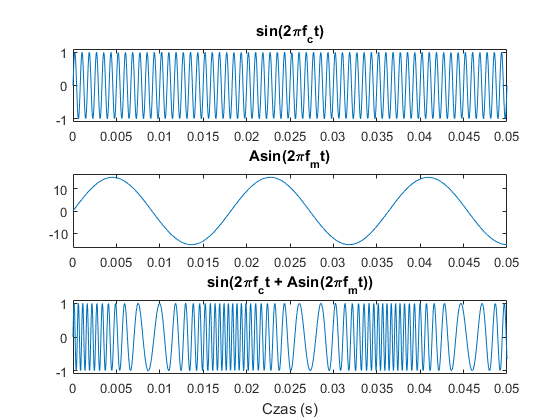
\includegraphics[width=12cm]{grafiki/fm_wykres1}
	\captionsetup{justification=centering}
	\caption{Prosty przykład sygnału zmodulowanego.}
	\label{rys:fm_wykres1}
\end{figure}

Wartość $\beta$ jest także określana mianem indeksu modulacji \cite{chowning}. Widmo sygnału poddanego modulacji częstotliwościowej składa się z prążka środkowego na częstotliwości nośnej oraz prążków bocznych. Prążki boczne są rozmieszczone symetrycznie względem częstotliwości nośnej i leżą na częstotliwościach $f_c \pm kf_m$, gdzie $k$ jest liczbą całkowitą. Moduł widma sygnału z powyższego przykładu przestawiony został na rysunku \ref{rys:fm_widmo}.

\begin{figure}[H]
	\centering
	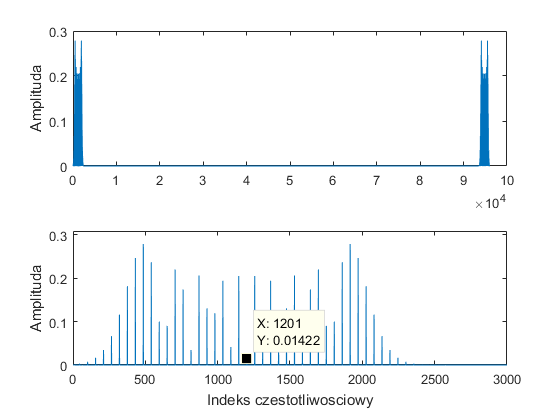
\includegraphics[width=10cm]{grafiki/fm_widmo}
	\captionsetup{justification=centering}
	\caption{Moduł widma sygnału zmodulowanego.}
	\label{rys:fm_widmo}
\end{figure}
Wartości poszczególnych prążków odpowiadają wartościom funkcji Bessela typu pierwszego $J_n(x)$, gdzie $n$ jest rzędem. Wykresy tych funkcji dla trzech pierwszych rzędów przedstawione są na rysunku \ref{rys:fm_bessel}.
\begin{figure}[H]
	\centering
	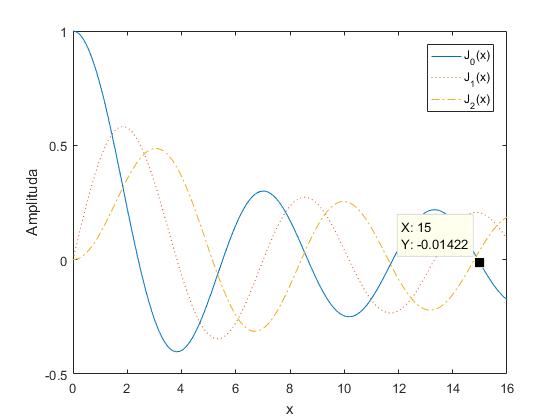
\includegraphics[width=10cm]{grafiki/fm_bessel}
	\captionsetup{justification=centering}
	\caption{Funkcje Bessela typu pierwszego.}
	\label{rys:fm_bessel}
\end{figure}

Moduł funkcji Bessela rzędu 0 w punkcie $\beta$ jest równy modułowi prążka na częstotliwości $f_c$. Moduł pierwszych prążków bocznych, tj. na częstotliwościach $f_c \pm f_m$ jest równy funkcji Bessela rzędu 1 w punkcie $\beta$. Postępując analogicznie można wyznaczyć moduły wszystkich prążków.